\section{ClangAutoMarker}

%----------------------------------------------------------------------
% Simplifying the AST
%----------------------------------------------------------------------

\subsection{Simplifying the AST}

\begin{frame}{Simplifying the AST}
\begin{itemize}
\item Mimic judgement process of human reader
\item Canonicalize logically similar structures
\end{itemize}
\end{frame}

\note{
\begin{itemize}
\item The first step after we let Clang parse the solution files into an AST is to simplify it
\item This serves two purposes
\begin{itemize}
\item First it tries to mimic the judgement process of a human reader
\item Second it canonicalize logically similar structures together so that even if they are written differently and get parsed into different AST, after similification their edit distance will be minimal if not 0
\end{itemize}
\end{itemize}
}

%----------------------------------------------------------------------

\begin{frame}{If-Statements}
\begin{overprint}
\onslide<1>
\lstinputlisting[language=C]{../media/code/simplify-if-neg-before.c}

\note{
\begin{itemize}
\item Let's start with a basic example: the if-statement
\item One common difference between student code, even if they are logically similar, is their condition can swap the order of true and false branches
\item Our simplification step would then canonicalize this if-statement by deleting the NOT node and flipping the
\end{itemize}
}

%----------------------------------------------------------------------

\onslide<2>
\lstinputlisting[language=C]{../media/code/simplify-if-neg-before.c}
\begin{tikzpicture}[remember picture, overlay, every to/.style={append after command={[draw=red]}}]
\draw [thick] (cross-a) to (cross-A);
\draw [latex-latex, thick, bend left, out=45, in=135] (swap-a.east) to (swap-A.east);
\end{tikzpicture}

%----------------------------------------------------------------------

\onslide<3>
\lstinputlisting[language=C]{../media/code/simplify-if-neg-after.c}
\end{overprint}
\end{frame}

\note{
\begin{itemize}
\item Here is the resulting if-statement
\item After simplification, we were able to canonicalize both this and the original form into the same AST; this greatly reduces their edit distances
\end{itemize}
}

%----------------------------------------------------------------------

\begin{frame}{Loops}
\begin{columns}
\column{0.5\textwidth}
\lstinputlisting[language=C, basicstyle=\scriptsize\ttfamily]{../media/code/simplify-loops-for-before.c}
\lstinputlisting[language=C, basicstyle=\scriptsize\ttfamily]{../media/code/simplify-loops-while-before.c}
\lstinputlisting[language=C, basicstyle=\scriptsize\ttfamily]{../media/code/simplify-loops-do-before.c}
\column{0.5\textwidth}
\lstinputlisting[language=C]{../media/code/simplify-loops-for-after.c}
\end{columns}
\end{frame}

\note{
\begin{itemize}
\item To give another example, here are 3 types of loops
\item For a human marker, they would generally skim over the loop condition and look at the contents; they are more interested that a student is looping over the CallStatement based on a condition that involves the number 5
\item As a result, our tool simplifies all 3 types, even though they are usually not logically equivalent
\end{itemize}
}

%----------------------------------------------------------------------

\begin{frame}{Variables}
\lstinputlisting[language=C]{../media/code/simplify-var.c}
\end{frame}

\note{
\begin{itemize}
\item Another thing we simplify in our AST are variables
\item Obviously we can't assume variable names across solutions are the same. Instead we opted for a simple system of canonicalizing variables into the set of function calls that read/write to them
\item In this example, since foo is on the LHS of the bar function call, we say that foo has been writen to by bar
\item Since x and y are parameters of bar, we say that they are read by bar
\item Finally, since y is passed by reference, we say that it's also written to by bar; while this isn't necessarily true, we make the worst case assumption because interprocedural analysis is both computationally expensive and complicated
\end{itemize}
}

%----------------------------------------------------------------------
% Pruning the AST
%----------------------------------------------------------------------

\subsection{Pruning the AST}

\begin{frame}{Pruning the AST}
\begin{itemize}
\item After simplification, we still have a lot of noise in our AST
\end{itemize}
\begin{overprint}
\onslide<1>
\lstinputlisting[language=C]{../media/code/pruning-useless-before.c}

\note{
\begin{itemize}
\item After simplifying and canonicalizing our AST, we still have a fair amount of junk nodes in our AST
\item For example, a human marker would not care about the implicit casts that a parser generates
\item As a result, we then need to postprocess our AST by deleting these useless nodes
\end{itemize}
}

%----------------------------------------------------------------------

\onslide<2>
\lstinputlisting[language=C]{../media/code/pruning-useless-before.c}
\begin{tikzpicture}[remember picture, overlay, every to/.style={append after command={[draw=red]}}]
\draw [thick] (cross-a) to (cross-A);
\draw [thick] (cross-b) to (cross-B);
\end{tikzpicture}

%----------------------------------------------------------------------

\onslide<3>
\lstinputlisting[language=C]{../media/code/pruning-useless-after.c}

\end{overprint}
\end{frame}

\note{
\begin{itemize}
\item Ultimately our goal is to distill our ASTs down to their barebones skeleton that capture the structure of our original solutions
\end{itemize}
}

%----------------------------------------------------------------------
% Computing TED
%----------------------------------------------------------------------

\subsection{Computing Tree Edit Distance}

\begin{frame}{Computing Tree Edit Distance}
\begin{block}{Tree Edit Distance (TED)}
The minimum total cost of the steps needed to change from a source tree to a destination tree.
\end{block}
\end{frame}

\note{
\begin{itemize}
\item Once we finished processing our AST, we can then move on to programatically compare them
\item The algorithm we will use is the Tree Edit Distance algorithm
\item This essentially calculates the minimum cost of the steps needed to change from a source tree to a destination tree
\end{itemize}
}

%----------------------------------------------------------------------

\begin{frame}{TED Example}
\begin{center}
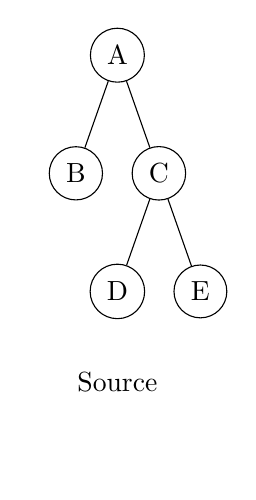
\begin{tikzpicture}[sibling distance=3em, every node/.style = {shape=circle, draw, align=center}]]
  \node{A}
    child { node{B} }
    child { node{C}
      child { node{D} }
      child { node{E} }
    }
    ;
  \node [below=3cm, align=flush center, text width=2cm, draw=none]{Source};
\end{tikzpicture}
\hspace{4em}
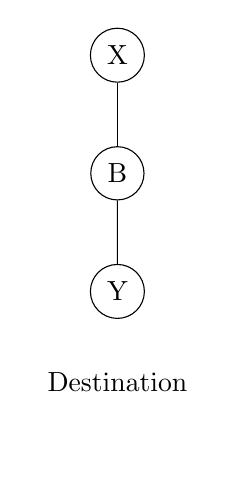
\begin{tikzpicture}[sibling distance=3em, every node/.style = {shape=circle, draw, align=center}]]
  \node{X}
    child { node{B}
      child { node{Y} }
    }
    ;
  \node [below=3cm, align=flush center, text width=2cm, draw=none]{Destination};
\end{tikzpicture}
\end{center}
\end{frame}

\note{
\begin{itemize}
\item Here is an example of how TED works
\item On the left is our source tree; on the right is our destination tree
\item In practice, these could be the student AST and reference AST
\end{itemize}
}

%----------------------------------------------------------------------

\begin{frame}{TED Example}{Delete}
\begin{center}
\begin{tikzpicture}[sibling distance=3em, every node/.style = {shape=circle, draw, align=center}]]
  \node{A}
    child { node{B} }
    child { node[draw=red, cross out, thick]{C}
      child { node[draw=red, cross out, thick]{D} }
      child { node[draw=red, cross out, thick]{E} }
    }
    ;
  \node [below=3cm, align=flush center, text width=2cm, draw=none]{Cumulative Cost: 3};
\end{tikzpicture}
\hspace{4em}
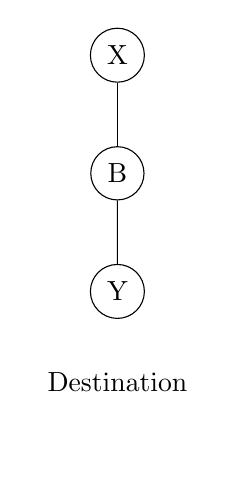
\begin{tikzpicture}[sibling distance=3em, every node/.style = {shape=circle, draw, align=center}]]
  \node{X}
    child { node{B}
      child { node{Y} }
    }
    ;
  \node [below=3cm, align=flush center, text width=2cm, draw=none]{Destination};
\end{tikzpicture}
\end{center}
\end{frame}

\note{
\begin{itemize}
\item One type of operation the TED algorithm will try is deleting existing nodes
\item The first step the algorithm might try is deleting the C,D,E nodes. Since we deleted 3 nodes, our cumulative cost thus far is 3
\item It is important to note that the cost can be varied
\item For example, we can penalize deleting variable nodes because it indicates that they are using excessive more variables than necessary
\end{itemize}
}

%----------------------------------------------------------------------

\begin{frame}{TED Example}{Insert}
\begin{center}
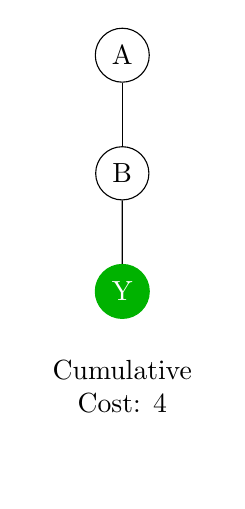
\begin{tikzpicture}[sibling distance=3em, every node/.style = {shape=circle, draw, align=center}]]
  \node{A}
    child { node{B} 
	  child { node[fill=black!30!green, draw=black!30!green, text=white]{Y} }    
    }
    ;
  \node [below=3cm, align=flush center, text width=2cm, draw=none]{Cumulative Cost: 4};
\end{tikzpicture}
\hspace{4em}
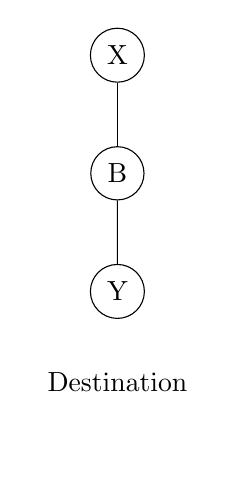
\begin{tikzpicture}[sibling distance=3em, every node/.style = {shape=circle, draw, align=center}]]
  \node{X}
    child { node{B}
      child { node{Y} }
    }
    ;
  \node [below=3cm, align=flush center, text width=2cm, draw=none]{Destination};
\end{tikzpicture}
\end{center}
\end{frame}

\note{
\begin{itemize}
\item The next type of operation is inserting new nodes
\item In our example, the algorithm then tries to insert a Y node increasing our cumulative cost to 4
\item In practice, we can for change the cost for inserting key function call nodes, meaning the student forgot to make these function calls themselves
\end{itemize}
}

%----------------------------------------------------------------------

\begin{frame}{TED Example}{Rename}
\begin{center}
\begin{tikzpicture}[sibling distance=3em, every node/.style = {shape=circle, draw, align=center}]]
  \node[strike out, draw=red, thick](a){A}
    child { node{B} 
	  child { node{Y} }    
    }
    ;
  \node at ([yshift=0.5cm, xshift=0.5cm]a) {X};
  \node [below=3cm, align=flush center, text width=2cm, draw=none]{Cumulative Cost: 5};
\end{tikzpicture}
\hspace{4em}
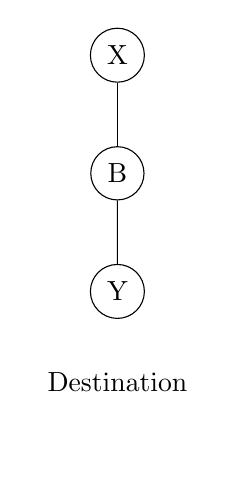
\begin{tikzpicture}[sibling distance=3em, every node/.style = {shape=circle, draw, align=center}]]
  \node{X}
    child { node{B}
      child { node{Y} }
    }
    ;
  \node [below=3cm, align=flush center, text width=2cm, draw=none]{Destination};
\end{tikzpicture}
\end{center}
\end{frame}

\note{
\begin{itemize}
\item Finally to get our destination tree, the algorithm can also rename existing nodes
\item Here we see that the total cumulative cost is 5
\end{itemize}
}

